\documentclass[english, 11pt]{article}
% \usepackage[T1]{fontenc}
% \usepackage[latin9]{inputenc}
\usepackage[top = 2cm, left = 2.5cm, right = 2.5cm, bottom = 2cm]{geometry}
\usepackage{enumitem}
\usepackage{amsmath}
\usepackage{amsfonts}
\usepackage{amstext}
\usepackage{mdframed}
\usepackage{graphicx}
% \usepackage{bbm}
\makeatletter
\@ifundefined{date}{}{\date{}}
\usepackage{tikz}
\usetikzlibrary{quotes, angles, decorations.markings, intersections}
\usetikzlibrary{calc,patterns,angles,quotes, 3d, intersections, positioning, shapes, automata, positioning}
\usepackage{wasysym}
\makeatother
\usepackage{babel}
\usepackage{color}
\usepackage{graphicx}
\usepackage{hyperref}
\hypersetup{
	colorlinks,
	citecolor=black,
	filecolor=black,
	linkcolor=black,
	urlcolor=black
}


\newcommand{\tbox}[1]{\noindent\fbox{\parbox{\textwidth}{#1}}}

\setlength{\parindent}{0pt}

\begin{document}

\textbf{CS 745 : Principles of Data and System Security} \hfill
\textit{Scribed by}: Kavin Arvind

\noindent\tbox{

\begin{center}
  \huge Lecture - 01 \\ % change lecture number
  \Large Topic:  History of Cryptography
\end{center}

}

\section*{Shifted cipher}
Each letter is Shifted by $k$ and sent. Eg- "A" is written as "A"+k (Shifted by k letters) and sent. \\
This is easy to decode as only 26 ( or 36 (if 0-9 nos are included)) possible $k$ are there and thus its easy to check each possibility.

\section*{Rolling by wooden stick}
A paper is rolled on to a stick and text is written. If seen normally, the letters would look fully shuffled, but if its rolled in the same way as it was written, it can be decoded.\\
eg- "MY NAME IS X" is written like
\begin{figure}[ht]
    \centering
        \begin{tabular}{ccccccccc}
            M &   &   &   & M &   &   &   & X\\
              & Y &   & A &   & E &   & S &  \\
              &   & N &   &   &   & I &   &  \\
        \end{tabular}
\end{figure}
\\
Thus its crypted as MMXYAESNI.

\section*{Mono-Substitution cipher}
We have a table where each letter is mapped to other letters and text is ciphered according to that. Here, we have here $26!$ ways of mapping and so its very difficult to try different possibilities. \\
This seems like an optimal solution, but there is a problem. In an average english text, each letter has a specific frequency of repetition. \\
Say letter "A" is coded to letter "K" (randomly). So frequency of letter K would be same as of the letter "A" in a normal text. So by this way, cipher text could possibly be decrypted.

\clearpage
\noindent\tbox{

\begin{center}
  \huge Lecture - 02 \\ % change lecture number
  \Large Topic:  History of Cryptography(Continuation.)
\end{center}

}

\section*{Homophonic Cipher}
The main problem of Mono-Substitution cipher is that, a character was substituted with only one alphabet and so the frequency didn't change.\\
What if its substituted with many characters to equalize the frequencies? \\
Say $S = \{A,B,..Z,0,1,..9,\epsilon, \alpha, \beta, \gamma, ...\}$ has usable symbols. \\
Say letter "A" has frequency $x\%$. We allot $\frac{x}{100} \times |S|$ number of symbols and are randomly substituted in the cipher text in place of "A".
This uniforms/balences the frequency among all the symbols and hence difficult to decrypt by frequency method. \\
But here, storing the mapping, encrypting, and decrypting are difficult.

\section*{Vigenere's Cipher}

What if we substitute "A" by any of the letters strategically? Vigenere created a table as shown below.

\begin{figure}[ht]
  \centering
      \begin{tabular}{|c|c|c|c|c|c|c|c|c|}
          \hline
            & A & B & C & D & ..\\
          \hline
          A & B & C & D & E & ..\\
          B & C & D & E & F & ..\\
          . &   &   &   &   &   \\
          . &   &   &   &   &   \\
          \hline
      \end{tabular}
\end{figure}
A keyword is chosen and correspondingly added to the text encrypt it. Eg -
\begin{figure}[ht]
  \centering
      \begin{tabular}{|c|ccccccccc|}
          \hline
          Actual text & M & Y & N & A & M & E & I & S & X \\
          keyword     & R & O & S & E & R & O & S & E & R \\
          \hline
          Cipher      & .. &   &   & F &   &   &   &   & \\
          \hline
      \end{tabular}
\end{figure}
Thus here, according to the position, same letter is encrypted to different letters and thus the frequencies are balenced.\\
Is it a good method then? \\
Words like "THE", "IS", etc repeat so much in english that its very likely that it is encrypted to the same cipher text due to same relative position w.r.t keyword. Calculating the repeated strings in ciphertext and observing the distance between them will give insigts about the length of keyword.
Length of keyword would be a factor of those distances and can be found out(say $l$). Now, characters $1,1+l,1+2l,..$ are derived from same column of the table. Hence they are like monostituted and now, frequencies can be calculated out to find the keyletters and hence keyword.

\section*{Mordern Cryptography}
\subsection*{Shannon's Cipher}
$\xi = (E,D)$ is a cipher system where $E(m,k) = c$($m$ is message, $k$ is key, $c$ is cipher text) is encyption funtion, and $D(c,k) = m$ is decryption funtion.

\subsection*{One Time Pad}
Say $m^l$ is a message of bits of length $l$, and key $k^l$ is key of same length generated randomly.
\[ E(m,k)= m^l \oplus k^l = c \]
\begin{align*}
  D(c,k) &= c^l \oplus k^l \\
  &= m^l \oplus k^l \oplus k^l \\
  &= m^l \\
\end{align*}
Provided key is generated completely random, and no part of key is known to Evasdropper, they can't decrypt it as probability of $c$ being 0 or 1 is independent of message itself. I.e,
\[ Prob(cipher = c | msg = m) = Prob(cipher = c | msg = m') \]
Hence, it is safe.
Disadvantages:
\begin{itemize}
  \item key is as big as message(or more)
  \item key should be sent safely. Otherwise its easily decrypted.
\end{itemize}
If key length is more, either its padded at the end and xored, or key is taken till the length of message and xored. \\
In general, if its not a bit string, the encryption can be taken as sum modulus like:
\[ E(m,k)= m^l + k^l \pmod{n} = c \text{  (if n=2, its just xor)} \]
\begin{align*}
  D(c,k) &= c^l - k^l \pmod{n} \\
  &= m^l + k^l - k^l \pmod{n}\\
  &= m^l \pmod{n}\\
\end{align*}

\clearpage
\noindent\tbox{

\begin{center}
  \huge Lecture - 03 \\ % change lecture number
  \Large Topic:  Perfect Secrecy and Shannon's information Theory
\end{center}

}
\section*{Perfectly secrecy}
\subsection*{OTP}
For a message to be perfectly secret, the Evasdropper should not be able to get any extra information from the ciphertext. So, \\
\begin{align*}
  P(M=m|C=c) &= P(M=m) \quad \text{[message = m, and ciphertext = c]} \\
  P_c(m) &= P(m) \\
  \frac{P(M=m|C=c)}{P(M=m)} &= \frac{P(C=c|M=m)}{P(C=c)} \\
  &= \frac{P(C=c|M=m)}{\sum_{m' \in M} P(C=c|M=m')P(M=m')} \\
\end{align*}
\[
\left[
\begin{aligned}
  P(C=c|M=m') &= P(K \oplus m' = c | M = m') \\
  &= P(K = c \oplus m'  | M = m') \\
  &= \frac{1}{2^l} \quad \text{[as key is selected randomly, probability that its $c \oplus m'$ is $1/2^l$]} \\
\end{aligned}
\right]
\]
\begin{align*}
  \frac{P(M=m|C=c)}{P(M=m)} &= \frac{P(C=c|M=m)}{\sum_{m' \in M} P(C=c|M=m')P(M=m')} \\
  &= \frac{1/2^l}{\sum_{m' \in M} (1/2^l)P(M=m')} \\
  &= \frac{1}{\sum_{m' \in M} P(M=m')} \\
  &= \frac{1}{1} \\
  P(M=m|C=c) &= P(M=m) \\
\end{align*}
Hence proved that it is perfectly secret. \\
But, what happens if key is repeated? Say a message said "Fire the gun" to a soldier which was ciphered to $c$ using key $k$, though an Evasdropper technically doesn't know the key, now he would see the soldier firing after getting message and so he can guess the message.
Using the ciphertext, he can get the $key = message \oplus cipher$ and if same key is used again, he would guess the message. Thus key can be used just once.\\
Also, if $M = {m_1='a',m_2='ab'}$ and,\\
if $c='x'$, $P_c(m_1) = 1$ and $P_c(m_2) = 0$ (This method reveals length of the message) \\
if $c='xy'$, $P_c(m_1) = 0$ and $P_c(m_2) = 1$.

\subsection*{Substitution cipher}
If $M = {m_1='aa',m_2='ab'}$ and,\\
if $c='xx'$, $P_c(m_1) = 1$ and $P_c(m_2) = 0$. \\
if $c='xy'$, $P_c(m_1) = 0$ and $P_c(m_2) = 1$. \\
Thus its not perfectly secret.

\subsection*{Addition OTP}

\begin{align*}
  D(c,k) &= c^l - k^l \pmod{n} \\
  &= m^l + k^l - k^l \pmod{n}\\
  &= m^l \pmod{n}\\
\end{align*}
Proof is very similar to as OTP.

\section*{Shannon's information Theory}
"No class on Friday" has more information/importance than "There is class on Friday" because having no class is a rare thing, and need to informed importantly. Having class is a regular thing and it doesn't carry much info.
So,
\begin{align*}
  \text{information} &\propto \frac{1}{\text{probability of occurance}} \\
  Info(x) &\propto \frac{1}{P(x)} \\
\end{align*}
Entropy of a message distibution($X$) is defined as:
\begin{align*}
  H(X) &= -\sum_{x \in X} P(x) \log_{2}(P(x)) \\
  &= \sum_{x \in X} P(x) \log_{2}(\frac{1}{P(x)}) \\
\end{align*}
Entropy is max when each of the messages has equal probability i.e, they are more uncertain. \\
Conditonal entropy of X, given Y is:
\begin{align*}
  H_Y(X)&= \sum_{X,Y} P(x,y) \log_{2}(\frac{1}{P_y(x)}) \\
  &= \sum_{Y} P(y) \sum_{X} P(x) \log_{2}(\frac{1}{P_y(x)}) \\
\end{align*}
If $C$ is the cipher text, and if $ H_C(M) \approx 0 $, then its easily breakable as it is not that uncertain.

\clearpage
\noindent\tbox{

\begin{center}
  \huge Lecture - 04 \\ % change lecture number
  \Large Topic: Key distributions
\end{center}

}

\section*{Symmetric Key Cryptography}
The methods we have seen so far including Substitution cipher, OTP, etc, are Symmetric key Cryptography as both the sender and receiver needs the same key to encrypt and decrypt the message. Here, the main difficulty was to exchage keys between both parties safely.\\
Its two types are \textbf{Stream Cipher} and \textbf{Block cipher} which we'll see later.

\section*{Assymetric key Cryptography}

Here, a pair of Keys $E_k$ and $D_k$ are created by a party which are related to each other in some sense.\\

\subsection*{Method 1: Secrecy Ensured}
Lets say, person $A$ wants to send a message to person $B$. Now, person $B$ created the pair of keys $E_B$ and $D_B$ and sends $E_B$ publically.
So, now $A$ encrypts message $m$ using $E_B$ to send cipher $c$.\\
Here, since $D_B$ is known only by person $B$, just $B$ can decrypt it and no one else. Thus here, secracy is ensured. But, cipher $c$ can be tapped and some other message $m'$ can be encrypted to $c'$ using public key $E_B$ by an Evasdropper and sent. So, here, authenticity is not ensured.

\begin{figure}[ht]
  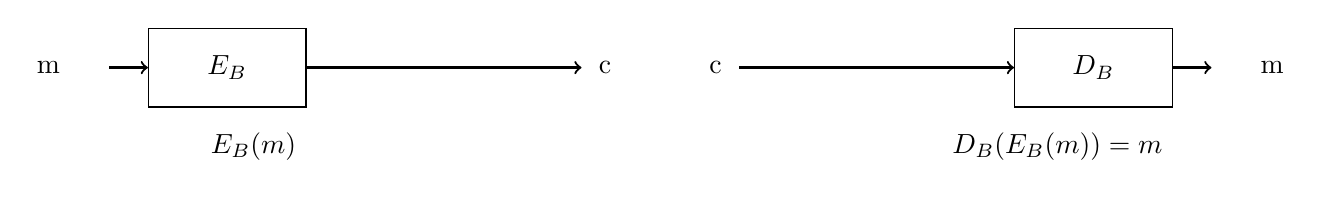
\begin{tikzpicture}
    % First set of text and boxes
    \node[anchor=east] at (0,0) {m};
    \node[draw, rectangle, minimum width=2cm, minimum height=1cm] (box1) at (2,0) {$E_B$};
    \node[anchor=east] at (3,-1) {$E_B(m)$};
    \node[anchor=west] at (8,0) {c};

    % Arrows
    \draw[->, thick] (0.5,0) -- (box1.west);
    \draw[->, thick] (box1.east) -- (6.5,0);

    % Second set of text and boxes
    \node[anchor=east] at (7,0) {c};
    \node[draw, rectangle, minimum width=2cm, minimum height=1cm] (box4) at (13,0) {$D_B$};
    \node[anchor=east] at (14,-1) {$D_B(E_B(m)) = m$};
    \node[anchor=west] at (15,0) {m};

    % Arrows
    \draw[->, thick] (8.5,0) -- (box4.west);
    \draw[->, thick] (box4.east) -- (14.5,0);

\end{tikzpicture}


  \centering   
\end{figure}

\subsection*{Method 2: Authenticity Ensured}
Lets say, person $A$ wants to send a message to person $B$. Now, person $A$ created the pair of keys $E_A$ and $D_A$ and sends $E_A$ publically.
So, now $A$ encrypts message $m$ using $D_A$ to send cipher $c$.\\S
Here, since $E_A$ is known by everyone including $B$, he can decrypt it using $E_A$. Thus here, authenticity is ensured as $D_A$ is private to person $A$ and only he/she can encrypt it. But, cipher $c$ can be decrypted by littrally everyone as $E_A$ is known publically. So security is not ensured.

\begin{figure}[ht]
  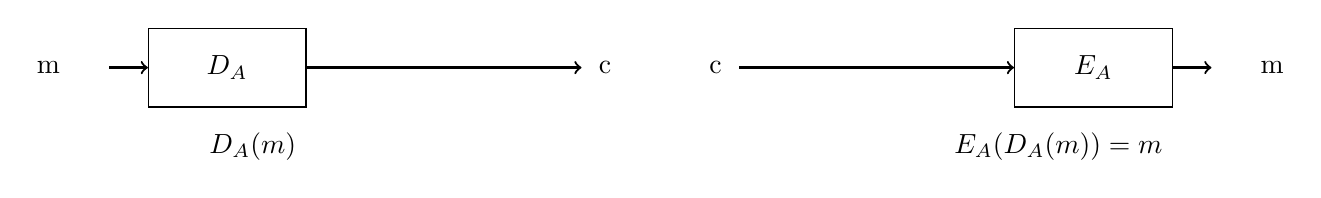
\begin{tikzpicture}
    % First set of text and boxes
    \node[anchor=east] at (0,0) {m};
    \node[draw, rectangle, minimum width=2cm, minimum height=1cm] (box1) at (2,0) {$D_A$};
    \node[anchor=east] at (3,-1) {$D_A(m)$};
    \node[anchor=west] at (8,0) {c};

    % Arrows
    \draw[->, thick] (0.5,0) -- (box1.west);
    \draw[->, thick] (box1.east) -- (6.5,0);

    % Second set of text and boxes
    \node[anchor=east] at (7,0) {c};
    \node[draw, rectangle, minimum width=2cm, minimum height=1cm] (box4) at (13,0) {$E_A$};
    \node[anchor=east] at (14,-1) {$E_A(D_A(m)) = m$};
    \node[anchor=west] at (15,0) {m};

    % Arrows
    \draw[->, thick] (8.5,0) -- (box4.west);
    \draw[->, thick] (box4.east) -- (14.5,0);

\end{tikzpicture}


  \centering   
\end{figure}

\subsection*{Method 3: Both Ensured}
What if we combine both the above methods to ensure both..\\
Lets say, person $A$ wants to send a message to person $B$.\\
Both of them creates pairs of keys $E_A$, $D_A$ and $E_B$, $D_B$ (and, $E_B$, $E_A$ are public).

\begin{figure}[ht]
  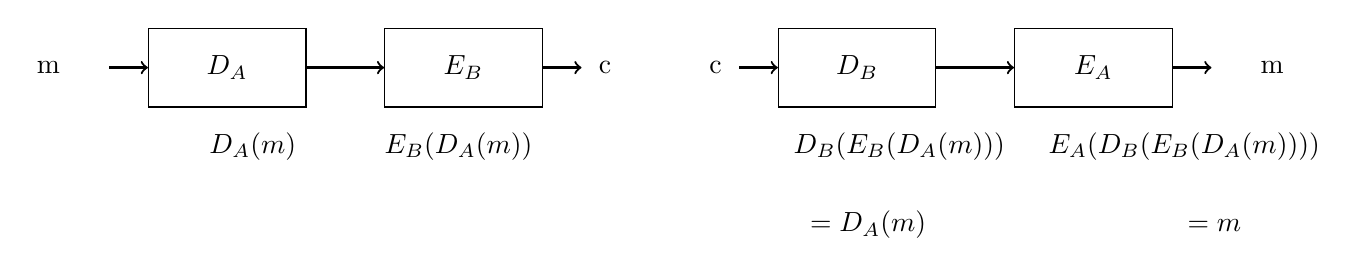
\begin{tikzpicture}
    % First set of text and boxes
    \node[anchor=east] at (0,0) {m};
    \node[draw, rectangle, minimum width=2cm, minimum height=1cm] (box1) at (2,0) {$D_A$};
    \node[anchor=east] at (3,-1) {$D_A(m)$};
    \node[draw, rectangle, minimum width=2cm, minimum height=1cm] (box2) at (5,0) {$E_B$};
    \node[anchor=east] at (6,-1) {$E_B(D_A(m))$};
    \node[anchor=west] at (8,0) {c};

    % Arrows
    \draw[->, thick] (0.5,0) -- (box1.west);
    \draw[->, thick] (box2.east) -- (6.5,0);

    % Second set of text and boxes
    \node[anchor=east] at (7,0) {c};
    \node[draw, rectangle, minimum width=2cm, minimum height=1cm] (box3) at (10,0) {$D_B$};
    \node[anchor=east] at (12,-1) {$D_B(E_B(D_A(m)))$};
    \node[anchor=east] at (11,-2) {$ = D_A(m)$};
    \node[draw, rectangle, minimum width=2cm, minimum height=1cm] (box4) at (13,0) {$E_A$};
    \node[anchor=east] at (16,-1) {$E_A(D_B(E_B(D_A(m))))$};
    \node[anchor=east] at (15,-2) {$ = m$};
    \node[anchor=west] at (15,0) {m};

    % Arrows
    \draw[->, thick] (8.5,0) -- (box3.west);
    \draw[->, thick] (box4.east) -- (14.5,0);
    \draw[->, thick] (box1.east) -- (box2.west);
    \draw[->, thick] (box3.east) -- (box4.west);

\end{tikzpicture}


  \centering   
\end{figure}
This suffices both authenticity and secracy. Here, its noteworthy that algorithm is known by everyone unlike the historical methods and just that the keys are kept secret.

\section*{Access Control}
Eg- MAC, DAC, RBAC, ABAC, etc are algorithms/methods used to enable access control. Lets understand this with an eg: \\
Lets say there is data stored in a database where only specific users can read and special users can edit it. Also, people should not be able to delete or scatter the information.
So, readers and modifiers should have their own specific keys.

\section*{Random Number Generation}
Its of two types:
\subsection*{True Random Number generator(TRNG)}
This is based on actual random events such as some hardware that changes drastically with outside conditions. It is truely random and can't be predicted.

\subsection*{Pseudo Random Number generator(PRNG)}
This is done algorithmic and could be predicted based on its previous values.

\end{document}